% Part: sets-functions-relations
% Chapter: relations
% Section: graphs

\documentclass[../../../include/open-logic-section]{subfiles}

\begin{document}

\olfileid{sfr}{rel}{grp}
\olsection{Graf}

\emph{Graf} yaiku diagram kang titik-titike---diarani
"simpul" utawa "verteks" (bentuk jamak ing basa Inggris
yaiku "vertices")---disambungake dening rusuk.
Graf minangka piranti kang umum banget ing matematika diskret
lan ilmu komputer. Graf migunani banget kanggo makili lan
nggambarake sesambungan lan struktur, saka bab nyata kayata
maneka jaringan nganti struktur abstrak kayata asil-asil
kaputusan kang bisa kedadeyan. Ing pustaka ana akeh jinis
graf kang beda, umpamane miturut apa rusuke mawa arah
utawa ora, duwe label utawa ora, apa bisa ana rusuk saka
simpul menyang simpul kang padha, luwih saka siji rusuk
antarane simpul kang padha, lan sapanunggalane.
\emph{Graf mawa arah} nduweni gayutan khusus karo relasi.

\begin{defn}[Graf mawa arah]
\emph{Graf mawa arah} $G = \tuple{V, E}$ yaiku
himpunan \emph{simpul}~$V$ lan himpunan
\emph{rusuk}~$E \subseteq V^2$.
\end{defn}

\begin{explain}
Miturut definisi kita, graf iku sawijining himpunan
bebarengan karo relasi ing himpunan kasebut.
Mesthi wae nalika ngrembug graf, lumrah yen graf
diwenehi wujud gambar: kita bisa nggambar graf
kanthi nyambungake rong simpul~$v_1$ lan $v_2$
nganggo panah yen lan mung yen $\tuple{v_1, v_2} \in E$.
Bedane relasi dhewe lan graf mung yen graf netepake
himpunan simpule, yaiku graf bisa duwe simpul kang
kapisah tanpa sambungan. Nanging kang wigati,
saben relasi~$R$ ing himpunan~$X$ bisa dianggep
graf mawa arah $\tuple{X, R}$, lan kosok baline,
graf mawa arah~$\tuple{V, E}$ bisa dianggep
relasi $E \subseteq V^2$ kanthi himpunan $V$
ditetepake kanthi cetha.
\end{explain}

\begin{ex}
Graf $\tuple{V, E}$ kanthi $V = \{1, 2, 3, 4\}$ lan
$E =\{\tuple{1,1}, \allowbreak \tuple{1, 2}, \allowbreak \tuple{1, 3},
\allowbreak \tuple{2, 3}\}$ katon kaya mangkene:
\begin{align*}
& 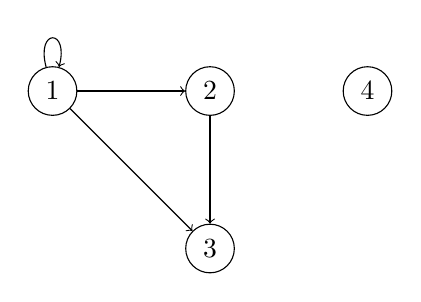
\begin{tikzpicture}[->,node distance=2cm]
  \node[draw,circle] (A) {$1$};
  \node[draw,circle] (B) [right of=A] {$2$};
  \node[draw,circle] (C) [below of=B] {$3$};
  \node[draw,circle] (D) [right of=B] {$4$};
  \draw (A) to [loop above]  (A);
  \draw (A) to  (B);
  \draw (A) to  (C);
  \draw (B) to  (C);
  \end{tikzpicture}
\intertext{Iki beda karo graf $\tuple{V', E}$ kanthi $V' =
  \{1, 2, 3\}$, kang katon kaya mangkene:}
& 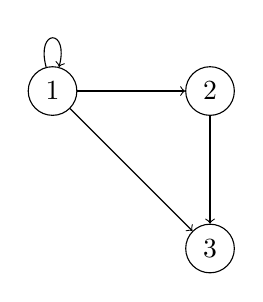
\begin{tikzpicture}[->,node distance=2cm]
  \node[draw,circle] (A) {$1$};
  \node[draw,circle] (B) [right of=A] {$2$};
  \node[draw,circle] (C) [below of=B] {$3$};
  \draw (A) to [loop above]  (A);
  \draw (A) to  (B);
  \draw (A) to  (C);
  \draw (B) to  (C);
  \end{tikzpicture}
\end{align*}
\end{ex}

\begin{prob}
  Anggepen relasi kurang saka utawa padha karo~$\le$
  ing himpunan $\{1,2, 3, 4\}$ minangka graf,
  banjur gambarna diagram kang cocog.
\end{prob}

\end{document}
